\documentclass[preprint,linenumbers,amsmath,amssymb,aps,prstab]{revtex4-1}%

\usepackage{dcolumn}% Align table columns on decimal point
\usepackage{bm}% bold math
\usepackage{siunitx}
\usepackage{pifont}% http://ctan.org/pkg/pifont
\newcommand{\cmark}{\ding{51}}%
\newcommand{\xmark}{\ding{55}}%
\usepackage{fancyvrb}
%\usepackage{booktabs}
%\usepackage{amsmath}
%\usepackage{amsfonts}
\usepackage{url}
%\usepackage{algorithm}
%\usepackage{algorithmic}
\usepackage{listings}
\newcounter{lstmain}
\setcounter{lstmain}{1}
\usepackage{graphicx,xcolor,enumitem}
\usepackage{booktabs}


\lstnewenvironment{code}[1][]
{ \vspace{0.3cm}\footnotesize{\textsc{Code Listing \thelstmain: #1}}
  \hspace{0.1cm} \hrulefill
  \lstset{language=C++, basicstyle=\ttfamily\scriptsize,
    keywordstyle=\color{blue}\bfseries,commentstyle=\color{mygreen},
    stringstyle=\color{red}
  }
}
{
  \hrule \vspace{0.3cm}
  \addtocounter{lstmain}{1}
}

\lstnewenvironment{codeln}[1][]
{\textbf{Code Listing} \hspace{1cm} \hrulefill \lstset{language=C++, basicstyle=\ttfamily\scriptsize, numbers=left, numberstyle=\tiny, stepnumber=1, numbersep=5pt, keywordstyle=\color{blue}\bfseries,commentstyle=\color{mygreen}, stringstyle=\color{red}}}
{\hrule\smallskip}

\lstnewenvironment{smallcode}[1][]
{\lstset{language=C++, basicstyle=\ttfamily\scriptsize, keywordstyle=\color{myblue}\bfseries,commentstyle=\color{mygreen}, stringstyle=\color{red}}}
{\smallskip}

\xdefinecolor{mygreen}{RGB}{0,220,0}
\xdefinecolor{myblue}{RGB}{26,150,255}


\begin{document}

\title{A parallel general purpose multi-objective optimization framework,
  with application to electron beam dynamics}

\author{N. Neveu}
\altaffiliation[Also at ]{Argonne National Laboratory, USA}%Lines break automatically or can be forced with \\

\author{L. Spentzouris}
\affiliation{Illinois Institute of Technology, Chicago, IL}

\author{A. Adelmann}
\email{andreas.adelmann@psi.ch}
\author{Y. Ineichen }
%\email{yves.ineichen@gmail.com}
\author{A. Kolano}
\altaffiliation[Also at ]{
	University of Huddersfield, West Yorkshire, United Kingdom and  CERN, Genf}
\author{C. Metzger-Kraus}
\affiliation{
	PSI, Villigen, Switzerland}%

\author{C. Bekas}
\author{A. Curioni}

\affiliation{IBM Research, Zurich, Switzerland }%

\author{P. Arbenz}
\affiliation{%
	Department of Computer Science, ETH Zurich, Switzerland}%

\date{\today}% It is always \today, today,
%  but any date may be explicitly specified


\maketitle


\section{Supplemental Material} \label{sec:introduction}

The following information provides additional details about the code implementation
used in the paper above. In the following sections, we will also use the notion of ``forward solver'' to indicate the beam dynamics simulation (i.e. task).

\subsection{Components of the Framework}

The basic assumption in simulation-based optimization is that a
  call to an expensive simulation software component present in the
  constraints or objectives is needed.
The framework is divided in three exchangeable components, as shown in
  Fig.~\ref{fig:opt-framework-layout}, to encapsulate the major behavioral
  patterns of the framework.
%
\begin{figure}
  \centering
  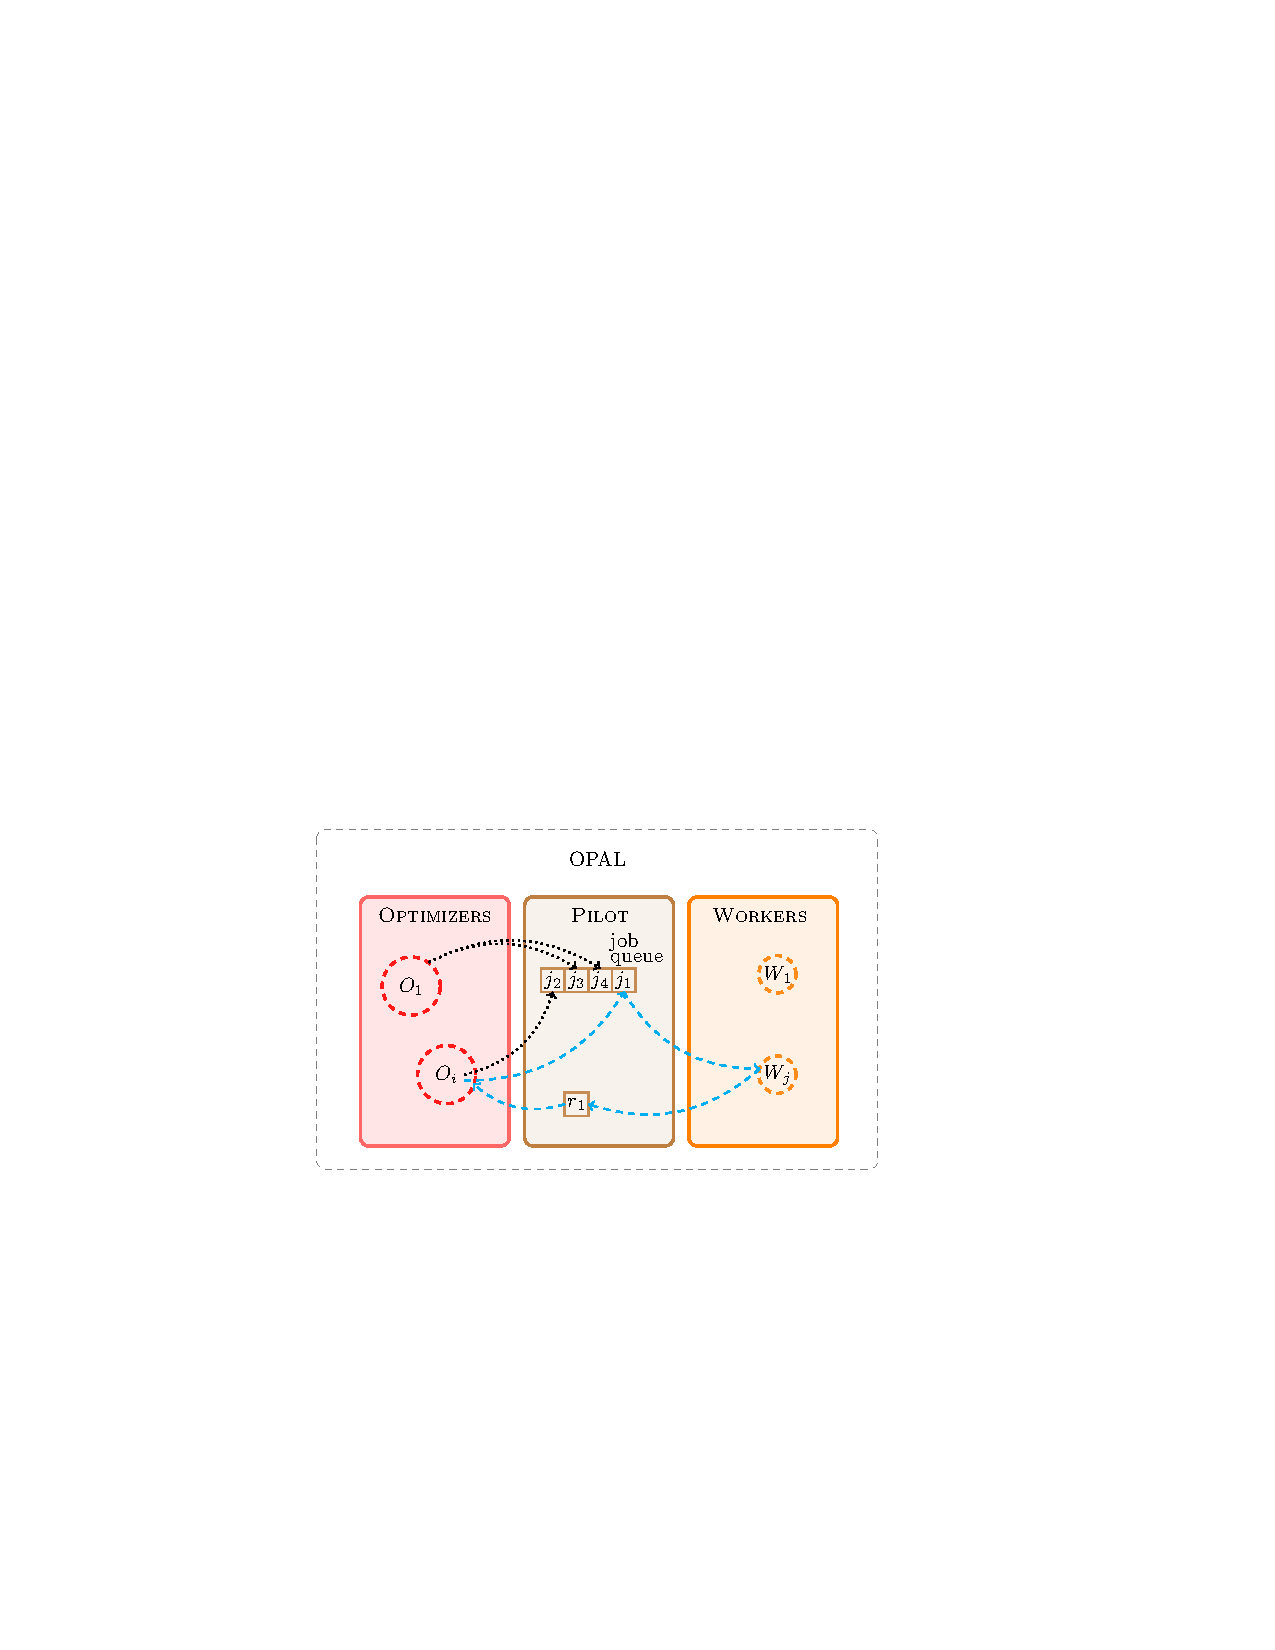
\includegraphics[width=0.7\linewidth]{opt-framework-layout}
  \caption{Schematic view of messages passed within the network between the
    three roles.
  The dashed cyan path describes a request (job $j_1$) sent from $O_i$ to the
  \textsc{Pilot} being handled by $W_j$. Subsequently the result $r_1$ is
  returned to the requesting \textsc{Optimizer} ($O_i$). $W_j$ are beam dynamics 
  simulations within OPAL.}
  \label{fig:opt-framework-layout}
\end{figure}

%
The \textsc{Pilot} component acts as a bridge between the optimizer and
  forward solvers, providing the necessary functionality to handle passing
  requests and results between the \textsc{Optimizer} and the
  \textsc{Simulation} modules.
The framework was implemented in \texttt{C++}, utilizing features like template
parameters to specify the composition of the framework.
``Default'' implementations are provided that can be controlled via command line options.
Due to its modular design, all components can be completely customized.

Every available MPI process will take up one of the three available roles (see
  Fig.~\ref{fig:framenetwork}):  one process acts as \textsc{Pilot}, the
  remaining processes are divided amongst \textsc{Worker} and
  \textsc{Optimizer} roles.
Both, the \textsc{Worker} and the \textsc{Optimizer} can consist of multiple
  MPI processes to exploit parallelism.
As shown in Fig.~\ref{fig:opt-framework-layout}, the \textsc{Pilot} is used
  to coordinate all ``information requests'' between the \textsc{Optimizer}
  and the \textsc{Worker}.
An information request is a job that consists of a set of design variables
  (e.g.~the genes of an individual) and a type of information it requests
  (e.g.~function evaluation or derivative).
The \textsc{Pilot} keeps checking for idle \textsc{Worker}s and assigns jobs
  in the queue to any free \textsc{Worker}.
Once the \textsc{Worker} has computed and evaluated the request its results
  are returned to the \textsc{Optimizer} that originally requested the
  information.

After a process gets appointed a role, it starts a polling loop to asynchronously
  check for appropriate incoming requests.
To that end a \textsc{Poller} interface helper class has been introduced.
The \textsc{Poller} interface consists of an infinite loop that checks
  periodically for new MPI messages.
Upon reception a new message is immediately forwarded to the appropriate
  handler: the \texttt{onMessage()} method.
The method is called with the \texttt{MPI\_Status} of the received message and
  a \texttt{size\_t} value specifying different values depending on the value
  of the \texttt{MPI\_Tag}.
The \textsc{Poller} interface allows the implementation of special methods
  (denoted \textit{hooks}) determining the behavior of the polling process,
  e.g.\ for actions that need to be taken after a message has been handled.
Every \textsc{Poller} terminates the loop upon receiving a special MPI tag.


\subsection{Implementing an Optimizer}

All \textsc{Optimizer} implementations have to respect the API shown in
Listing 1.

%\noindent\begin{minipage}{0.48\textwidth}
\begin{code}[Optimizer API]
virtual void initialize() = 0;

// Poller hooks
virtual void setupPoll() = 0;
virtual void prePoll() = 0;
virtual void postPoll() = 0;
virtual void onStop() = 0;
virtual bool onMessage(MPI_Status status,
                       size_t length) = 0;
\end{code}
%\end{minipage}

All processors running an \textsc{Optimizer} component call the
  \texttt{initialize} entry point after role assignment in the
  \textsc{Pilot}.
The implementation of \texttt{initialize} must set up and start the poller and
  the optimization code.
Since an optimizer derives from the \texttt{Poller} interface, predefined
  hooks can be used to determine the polling procedure.
Hooks can be implemented as empty methods, but the \texttt{onMessage}
  implementation should reflect the optimization part of the protocol for
  handling events from the \textsc{Pilot}.
A special set of communicator groups serves as communication channels to the
  \textsc{Pilot}, its job queue, and processes supporting the
  \textsc{Optimizer} component.


\subsection{Implementing a Forward Solver}

In most cases, forward solver implementations are simple wrappers to run
  an existing ``external'' simulation code using a set of design variables as
  input. In the case of the OPAL integration, the \texttt{main} function is
  playing the role of the ``forward solver''. To underline the general nature of our framework's software design, 
  in a similar project, the described methods are used for cavity shape optimisation based on \cite{ARBENZ2008381}. 
As for the \textsc{Optimizer} component there exists a base class, labeled
  \texttt{Simulation} as common basis for all \textsc{Simulation}
  implementations.
In addition, this component also inherits from the \texttt{Worker} class,
  already implementing the polling protocol for default worker types.
As shown in the API in Listing 2, the \texttt{Worker} class expects an
  implementation to provide implementations for three methods.

\begin{code}[Simulation API]
virtual void run() = 0;
virtual void collectResults() = 0;
virtual reqVarContainer_t getResults() = 0;
\end{code}

First, upon receiving a new job, the \texttt{Worker} will call the \texttt{run} 
method on the \textsc{Simulation} implementation.
This expects the \textsc{Simulation} implementation to run the simulation in a 
\textit{blocking} fashion, meaning the method call blocks and does not return
until the simulation has terminated.
Subsequently, the \texttt{Worker} calls \texttt{collectResults}, where the
\textsc{Simulation} prepares the result data, e.g. parsing output files,
and stores the requested information in a \texttt{reqVarContainer\_t} data structure.
Finally, the results obtained with \texttt{getResults} are sent to the \textsc{Pilot}. 
As before, the serialized data is exchanged using MPI point-to-point communication using a specific set of communicators.


\subsection{Specifying the Optimization Problem}

We aimed at an easy and expressive way for users to specify multi-objective optimization problems.
Following the principle of keeping metadata (optimization and simulation input data) together, 
we decided to embed the optimization problem specification in the simulation input file by 
prefixing it with special characters, e.g. as annotations prefixed with a special character.
In some cases, it might not be possible to annotate the simulation input file.
By providing an extra input file parser, optimization problems can be read from stand-alone files.
To allow arbitrary constraints and objective expressions, such as
%
%{0.2cm}
\begin{Verbatim}[fontsize=\scriptsize]
  name: OBJECTIVE,
        EXPR="5 * average(42.0, "measurement.dat") + ENERGY";
\end{Verbatim}
%\vspace{0.2cm}
%
\noindent
an expression parser using Boost Spirit~\cite{boost} was implemented.
In addition to the parser, we need an evaluator able to evaluate an expression,
given a parse tree and variable assignments to an actual value.
Expressions arising in multi-objective optimization problems usually evaluate
to booleans or floating point values.
The parse tree, also denoted abstract syntax tree (AST), is constructed recursively while an expression is parsed.
Upon evaluation, all unknown variables are replaced with values, 
either obtained from simulation results or provided by other subtrees in the AST.
In this stage, the AST can be evaluated bottom-up and the desired result is
  returned after processing the root of the tree.

To improve the expressive power of objectives and constraints, a
  simple mechanism to define and call custom functions in expressions was introduced.
Using simple functors, to compute an
  average over a set of data points, enriches expressions with custom
  functions.
Custom function implementations overload the \texttt{()} parenthesis operator.
The function arguments specified in the corresponding expression are stored in
  a \texttt{std::vector} of Boost variants~\cite{boost2} that can be
  booleans, strings or floating point values.

All custom functions are registered with expression objects.
This is necessary to ensure that expressions know how they can resolve
  function calls in their AST.
As shown in Listing 3 this is done by creating a collection of Boost
  functions~\cite{boost3} corresponding to the
  available custom functions in expressions and passing this to the
  \textsc{Pilot}.

%\noindent\begin{minipage}{\textwidth}
\begin{code}[Creating function pointer for registering functor]
functionDictionary_t funcs;
client::function::type ff;
ff = average();
funcs.insert(std::pair<std::string, 
		client::function::type> 
       		("my_average_name", ff));
\end{code}
%\end{minipage}

A set of default operators, corresponding to a mapping to \texttt{C} math
  functions, is included in the dictionary by default.
This enables an out of source description of optimization problems containing
  only simple math primitives.


\subsection{Parallelization} \label{sec:parallelization}

The parallelization is defined by a mapping of the roles introduced above to
  available cores.
Command-line options allow the user to steer the number of processors used in
  worker and optimizer groups.
Here, we mainly use the command-line options to steer the number of processors
  running a forward solver.

One major disadvantage of the master/slave implementation model is the fast
  saturation of the network links surrounding the master node.
In \cite{bctg:09} authors observe an exponential increase in hot-spot latency
  with increasing number of workers that are attached to one master process.
The limiting factor is the number of outgoing links of a node in the
  network topology. For a few workers, the links surrounding a
  master process are subject to congestion.
This effect is amplified further by large message sizes.

To that end we implemented a solution propagation based on rumor networks 
(see \cite{bgps:06,ayss:09}) using only one-sided communication.
This limits the number of messages sent over the already heavily used links
surrounding the master node and helps to prevent the use of
global communication. Using information about the interconnection network topology and the
application communication graph, the task of assigning roles helps to further
improve the parallel performance.



\section{FORWARD SOLVER} \label{sec:forward-solver}

The framework contains a wrapper implementing the API mentioned in
  Listing 1 for using \textsc{OPAL}~\cite{opal} as the forward solver.
\textsc{OPAL} provides different trackers for cyclotrons and linear
  accelerators with satisfactory parallel performance. 
With access to the \textsc{OPAL} forward solver, the framework is able to
  tackle a multitude of optimization problems arising in the domain of
  particle accelerators.
  The framework is also integrated into \textsc{OPAL} so that users can 
  define optimization problems within an input file, requiring no 
  additional knowledge or installation of the API to use it.

If the objectives and constraints are simple arithmetical expressions, 
the \texttt{FunctionEvaluator} simulator can be used.
Using functors and the default expression primitives, 
multi-objective optimization problems can be specified, 
i.e.\ the benchmark problem presented in \cite{hbwh:05}:
%

	\begin{widetext}
		\begin{align} \label{eqn:bench}
		\text{min} & \left[ 1 - \exp \left( -1 \left(
		\left(x_1 - \frac{1}{\sqrt{3}} \right)^2 +
		\left(x_2 - \frac{1}{\sqrt{3}} \right)^2 +
		\left(x_3 - \frac{1}{\sqrt{3}} \right)^2 \right)\right), \right. \\
		\vspace{3em} 
		& \left. 1 - \exp \left( -1 \left(
		\left(x_1 + \frac{1}{\sqrt{3}} \right)^2 +
		\left(x_2 + \frac{1}{\sqrt{3}} \right)^2 +
		\left(x_3 + \frac{1}{\sqrt{3}} \right)^2 \right)\right) \right]^T \nonumber \\
		\vspace{3em} \nonumber \\
		\text{s.t.} \quad & \quad -1 \le x_i \le 1, \quad i=1,2,3 \nonumber
		\text{.} \nonumber
		\end{align}
	\end{widetext}



\section{Example Optimization File}

This examples serves to show how a user can 
set up a multiobjective optimization run 
within an OPAL input file. 

The code that follows was used to perfrom ex-1 in Section~\ref{sec:experiments}.



\bibliography{paper}

\end{document}


